\documentclass{article}
\usepackage[utf8]{inputenc}
\usepackage{graphicx}
 
\begin{document}
\maketitle
\begin{center}

\author{Group D\\
We Works\\ \textbf{Magpie Composite Textile Ltd}\\ Group Members(4)-\\Name: Md Eyamin Molla \\ ID-19202103209(44)\\ Name: Md Rakibur Rahman Zihad\\ ID: 19201103082(43)\\ Name: Md Mohibbullah\\Id:19201103101\\ Name: Nahian Islam\\ID : 19201103028\\
Submitted to\\ Most.Jannatul Ferdoud, Lecturer
}
  
\newpage
\title{\huge Magpie Composite Textile Ltd\\
\small Bangladesh garments industry\\
}
\end{center}
\begin{center}
    
\huge \textbf {Acknowledgment}
\end{center}
We would like to pay our gratitude to the Almighty Allah who created us with all the abilities
to understand analysis and develop the process with patience. We are thankful to our project
teacher Most. Jannatul Ferdous, Lecturer, Department of CSE, Bangladesh University of
Business and Technology for his professional guidance and motivation during the work of this
project which is a major part of it. Without his valuable support and guidance, this project
could not reach this level of development from our point of view.
We would like to thank all the Faculty members, Department of CSE, Bangladesh University of
Business and Technology for their valuable time spend in requirements analysis and evaluation
of the project work. We would like to express our sincere and warm gratitude to all those who
have encouraged us directly, provided mental encouragement and criticized our work in several
phases during the development of this project and for preparing this project indirectly.
\newpage
\begin{center}
    \huge \textbf{Abstract}
\end{center}
Bangladeshi Garment Industry is the largest industrial sector of the country. Though the history of Readymade Garment Industry is not older one but Bangladeshi clothing business has a golden history. Probably it started from the Mughal age in the Indian subcontinent through Dhakai Musline. It had global reputation as well as demandable market around the globe especially in the European market.
After the industrial revolution in the west, they were busy with technological advancement & started outsourcing of ready made garments to meet up their daily demands. Many LDC's took that chance & started ready made garment export at that markets. As an LDC Bangladesh took this chance enjoyed quota & other facilities of them. Thus ready made garment industry started to contribute in our economy from late eighties (1977).
The history of the garment industry dates back to 1977 when the first consignment was exported to then-West Germany by Jewel Garments. The number of units, however, remained a meager 46 until the end of 1983. From a humble beginning the sector has thus made phenomenal growth over the last two decades, the number of units growing to around 4500. The RMG industry achievement is noteworthy, particularly for a country plagued with poor resource endowments and adverse conditions for industrialization. Exports increased from approximately 32 million US dollars in 1983/84 to 1.4 billion dollars in 1992/93. In 1987/88, the RMG export share surpassed that of raw jute and allied products. The figure further rose to 5.7 billion dollars in 2003/04, representing a contribution of about 75 percent of the country's total export earnings in that year. The employment generated by the sector is estimated to be around 1.5 million workers.
Several factors account for the outstanding successes of the RMG industry in Bangladesh. At the same time this industry had faced & till facing many problems also. These problems & prospects of RMG industry in Bangladesh is my topic to find out as well as to make critical analysis on these. The importance of my study has been raised up by recent labor unrest in RMG sector.
To analyze this board topic a took fulltime guidance from my dissertation guide Mr. A. K. M. Abduj Jaher in preparing questionnaire, operating field survey, presenting the survey report as well as constructing the report as a whole. So I am grateful to him.
Here I use data from different sources like, BGMEA, BKMEA, CPD, World Bank, UNDP, Lmd Journal Published by Australian National University, CIA Report, ADB, Bureau of Economic Research - University of Dhaka, The University of Chicago Press & many other sources stated in reference section. Thus I am obliged to all of them at the same time I would like to offer my warm thanks to all of them.
Many Garments owners, workers, & buyers have helped us by providing their valuable opinion on the topic or through interviews. So we are grateful to them for helping me by providing primary data. Again I would like to offer my warm thanks to all of them for helping me a lot in the construction of this dissertation report.
\newpage
\begin{center}
    \huge \textbf{Declaration}
\end{center}
We hereby declare that the work presented in the project report entitled Outliers by using
Boxplot submitted in partial fulfillment of the requirements for the degree of Bachelor of Science
in Computer Science and Engineering of Bangladesh University of Business and Technology
(BUBT) is our own work.
The matter embodied int his project report has not been submitted elsewhere by anybody for
the award of any degree.
\newpage
\tableofcontents
\newpage
\section{Introduction}
The textile and clothing industries provide a single source of growth in Bangladesh's rapidly developing economy.
Exports of textiles and garments are the principal source of foreign exchange earnings.The tremendous success of garment exports from Bangladesh over the last two decades has surpassed the most optimistic expectations.Today the apparel export sector is a multi-billion-dollar manufacturing and  export industry in the country. The overall impact of the garment exports is certainly one of the most significant social and economic developments in contemporary Bangladesh.With over one and a half million women workers employed in semi-skilled and skilled jobs producing clothing for exports, the development of the apparel export industry has had far-reaching implications for the society and economy of Bangladesh.
\begin{center}
     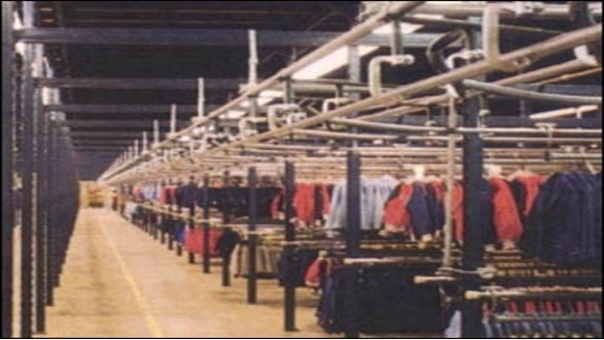
\includegraphics[width=\textwidth]{img/img1.png}
\end{center}

\subsection{Project Overview}
\begin{itemize}
\item The garment industry of Bangladesh has been the key export division and 
main source of foreign exchange for the last 25 years.
\item At present, the country generates about 5 billion worth of products each year by exporting garments.
The industry provides employment to about 3 million workers of whom 90 per-
cent are women.
\item Two non-market elements have performed a vital function in
confirming the garment industry’s continual success; these elements are\\
(a) quotas under Multi-Fiber Arrangement1 (MFA) in the North American
market and\\
(b) special market entry to European markets. The whole procedure is strongly
related to the trend of relocation of production.

\item The global economy is now controlled by the transfer of production where firms of developed countries swing their attention to developing countries. The new representation is centered on a core-periphery system of production, with a comparatively small center of per- moment employees dealing with finance, research and development, technological institution and modernization and a periphery containing dependent elements of the production procedure.

\item Reducing costs and increasing output are the main
causes for this disposition. They have discovered that the simplest way to under-
the charge is to move production to a country where labor charges and production
costs are lower. Since developing nations provide areas that do not impose costs
like environmental degeneration, this practice protects the developed countries
against the issues of environment and law.

\end{itemize}


\subsection{Why this is chossen?}
\begin{itemize}
\item There is a huge discrepancy between the way our young generation is being
taught in educational institutions, the kind of knowledge and skills needed to
work in the garment industry and move the industry forward in the future.
\item Many young people in our country are looking for
employment in the garment industry after finishing their studies. On the other
hand, a large number of foreigners are working in our garment industry at high
salaries. This means that the garment industry lacks the required number of
skilled manpower against the demand. The garment industry will have to face
many challenges in the future.
\item We need to prepare now to face those challenges.
We firmly believe that the current education system in our country will play
a helpful role in meeting the challenges of the future if we can fill the gaps in
education related to the garment industry.
   
\end{itemize}

\subsection{Problem Introduction}
\begin{itemize}
    \item Color Problem:
    
     The color problem is that the color of the garment does not match the sample given by the buyer.
     \item Printing Quality Problem:

    The buyer provided a quality print to create the sample. After making the sample, if the print quality of the buyer does not match the print quality of the sample, then it is called the Printing Quality Problem.\\
    \item Care Label Problem:
    The care label that is used when making ready-made garment samples. If any information is wrong in that care level, it is called care label problem.
Care label problems are common
Using another buyer's care label.
The size of the care label is getting bigger and smaller.
In general, the problem with care labels is that the instructions on the care label are incorrect.
\item Accessories Problem:

Many types of accessories are used to make garment samples. It is not possible to make a garment sample completely without these accessories.
So the problem is if the accessories are given differently without sampling the accessories according to the demand of the buyer, again if the quality of the accessories is not completed.
\item Brand Levelling Problem:

This problem occurs when using a brand level given by another buyer without using the brand label given by the buyer while making the garment sample or if the information given at the brand level is not correct.
\item Style Problem:

When the buyer gives the merchandiser the artwork of the prepared sample, it is mentioned what style will be in the sample.
This problem occurs when the sample prepared in the garments does not match the artwork style given by the buyer.
 \item Quality Problem:

Sample Quality Problem This problem occurs when various types of faults or errors are found in the prepared sample.
\item Measurement Problem:

This measurement problem is most important in the sample department. Because if there is any problem in the measurement of the sample, the buyer will never buy it.

\end{itemize}
\newpage
\subsection{Objective}
\begin{itemize}
    \item  Bangladesh is a developing country where the industry has not fully developed.
However, among the industries that have been developed in Bangladesh, the gar-
the mint industry is the main one.
\item Bangladesh’s garment industry has a monopoly
on export trade. Not only export trade but also the employment of millions of people is involved. Bangladesh has a reputation in the garment sector all over the
world. But at present, this world-class garment industry is facing a crisis today.
The image of Bangladesh’s garment industry abroad is under threat due to the
economic downturn, competition in the free-market economy, and cancellation
of GSP facilities.
\item Firmly believes that the current education system in our country will play a helpful role in meeting
the challenges of the future if we can fill the gaps in education related to the
garment industry.
\end{itemize}

\newpage
\section{Analysis of the system}
Use case diagrams are a set of use cases, actors, and their relationships. They represent the
use case view of a system.
A use case represents a particular functionality of a system. Hence, use case diagram is used
to describe the relationships among the functionalities and their internal/external controllers.
These controllers are known as actors.
Use case diagrams are considered for high level requirement analysis of a system. When the
requirements of a system are analyzed, the functionalities are captured in use cases.Actors can
be human user, some internal applications, or may be some external applications. When we
are planning to draw a use case diagram, we should have the following items identified.
\begin{itemize}
    \item Functionalities to be represented as use case
\item Actors
\item Relationships among the use cases and actors
\item The name of a use case is very important. The name should be chosen in such a way so
that it can identify the functionalities performed.
\item Do not try to include all types of relationships, as the main purpose of the diagram is to
identify the requirements.
\end{itemize}
\newpage
\subsection{Use Case Diagram}
A Use Case diagram models the dynamic behavior of the system when it is operating. It highlights the high-level requirements of the system. It is modeled to represent the outside view of the system.
\subsection{Existing System Use Case Diagram}
\begin{figure}[h]
    \centering
    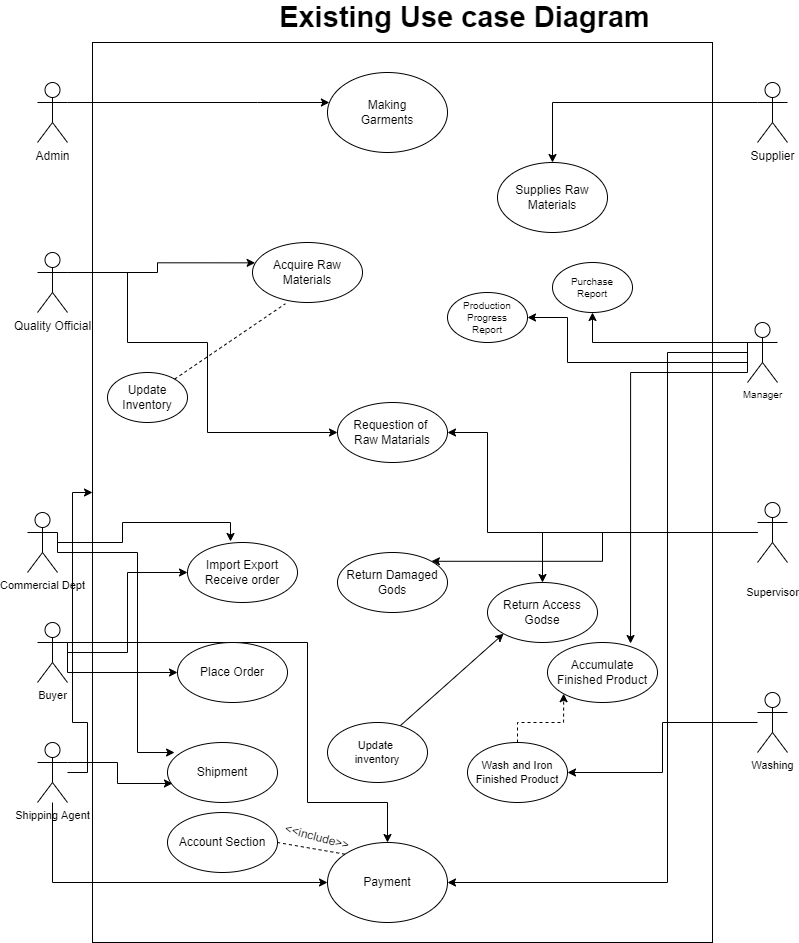
\includegraphics[width=13cm,height=13cm]{img/existingusecas.png}
    \caption{Existing System Use Case Diagram}
    \label{fig:my_label}
\end{figure}
\newpage
\subsection{Proposed Use Case Diagram}
\begin{figure}[h!]
    \centering
    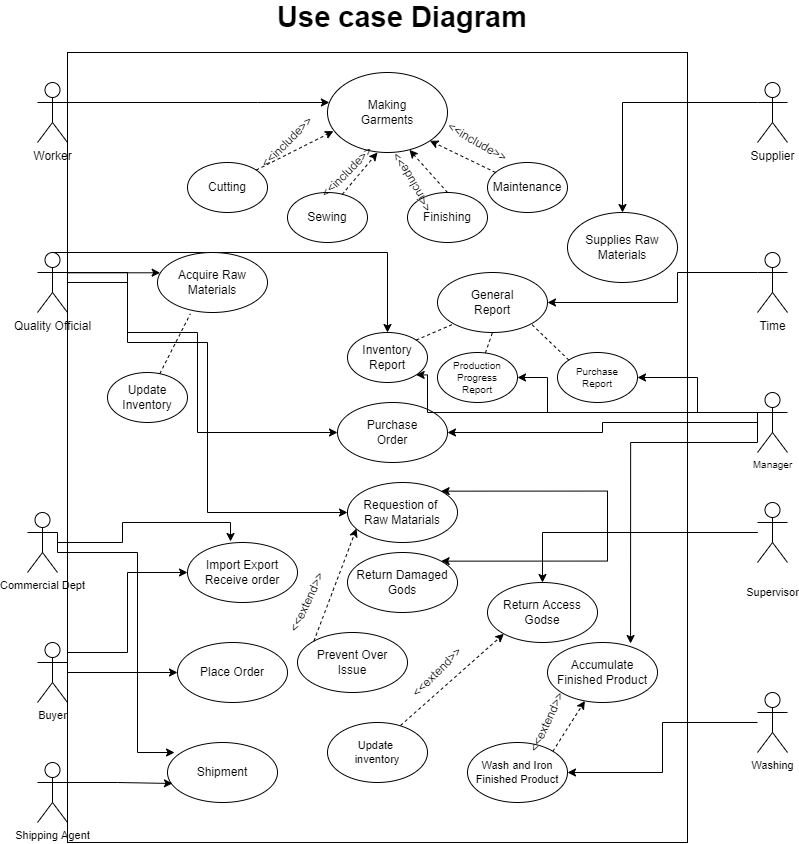
\includegraphics[width=10cm]{img/usecachdia.png}
    \caption{Use Case Diagram}
    \label{fig:my_label}
\end{figure}
\newpage
\subsection{Existing System DFD Diagram}
\begin{figure}[h]
    \centering
    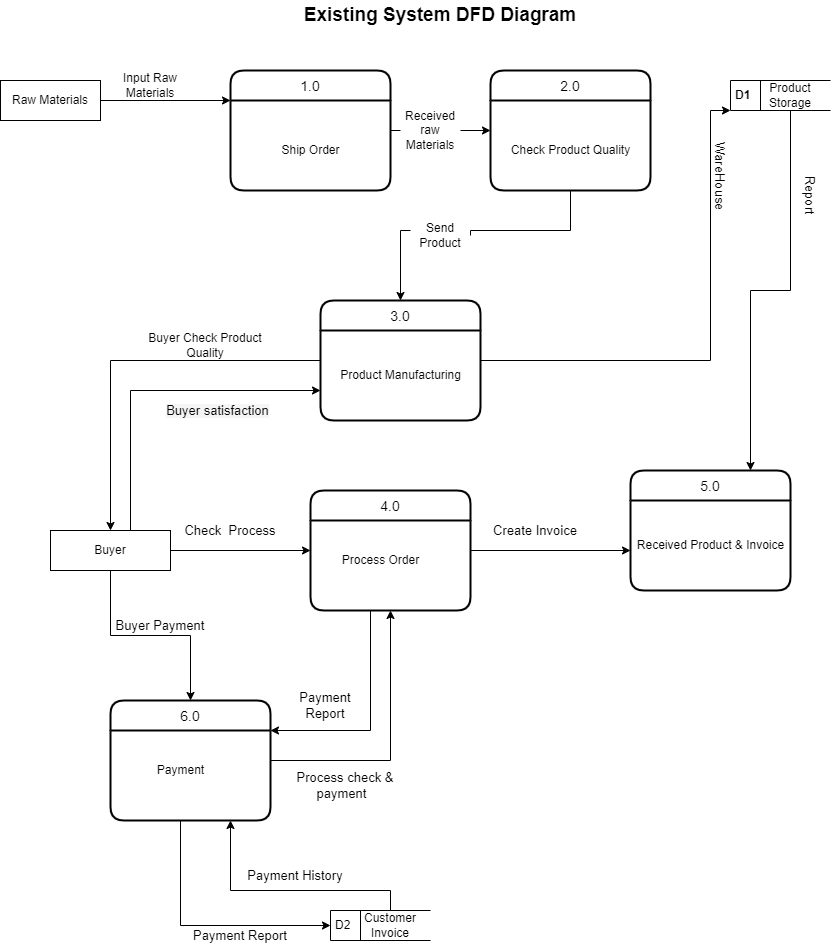
\includegraphics[width=10cm]{img/exisitingdfd.png}
    \caption{Existing System DFD Diagram}
\end{figure}
\newpage
\subsection{Proposed DFD Diagram}
\begin{figure}[h!]
\centering
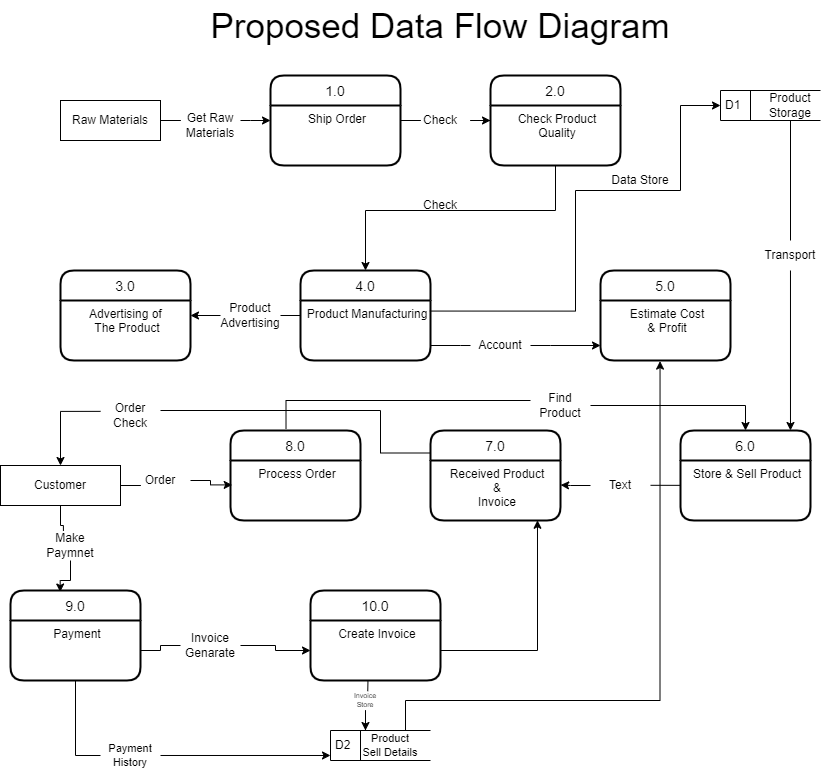
\includegraphics[width=13cm]{img/dfd diagram.drawio.png}
\caption{Data Flow Diagram}
\label{dfd}
\end{figure}
\newpage
\subsection{Existing System Context Diagram}
\begin{figure}[h]
    \centering
    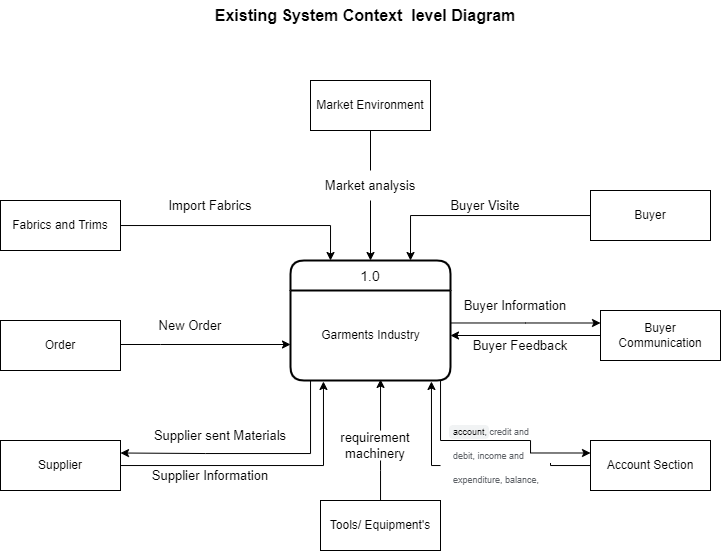
\includegraphics[width=13 cm]{img/exiting context diagram.png}
    \caption{Existing System Context Level Diagram}
    \label{fig:my_label}
\end{figure}
\newpage
\subsection{Proposed Context Diagram}
\begin{figure}[h]
    \centering
    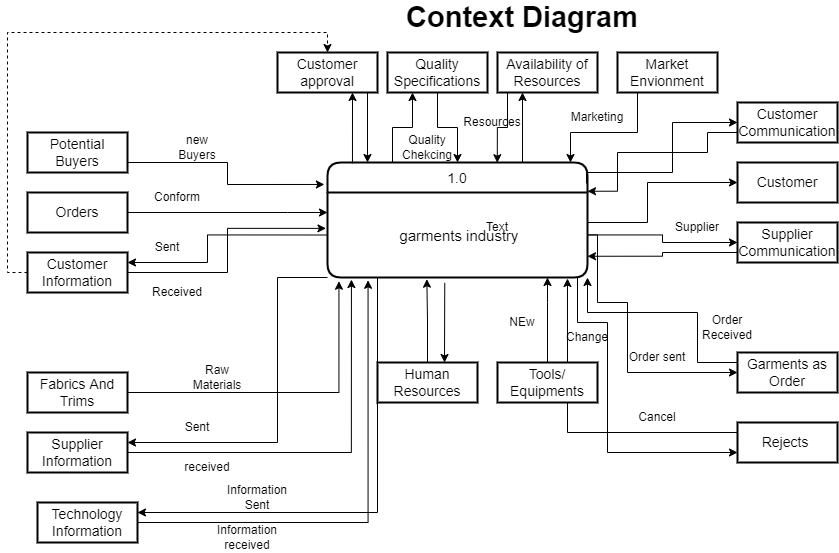
\includegraphics[width=13 cm]{img/contextdiag.png}
    \caption{Proposed Context Diagram}
    \label{fig:my_label}
\end{figure}
\newpage
\newpage
\section{Feasibility Analysis}
 Feasibility analysis evaluates all key factors pertinent to a project, including the economic, technological, and legal aspects and project time frame — all of which help predict the likelihood of project success. Feasibility analysis, also known as Feasibility Study, intends to equitably and logically examine the pros and cons of an existing or a proposed business, dangers related to the venture, required resources to carry out the operations, and eventually the probability of success. Feasibility analysis gives a clear picture of the budget required and the returns that can be expected. A feasibility study is not restricted to forecasting monetary benefits. It can be used for other purposes depending upon 10 the target of the project and the industry to which it belongs. Introduction to importation viability Importation viability is an assessment process with the help of which an importer can take the decision whether he or she is ready to take the risk. It helps the importer whether the product or goods viable or profitable to import to the desired location. This include local economic and scion-economic factors physical conditions, political and legal conditions as well as cultural conditions such as aesthetics, attitudes and belief, religion, material culture and language. The process of feasibility analysis includes three specific steps. In step 1 the project evaluation using selected capabilities of feasibility’s of the analysis i.e., evaluation of legal capabilities, evaluation of operational capabilities, evaluation of economic capabilities, evaluation of capabilities related to the schedule and evaluation of system and technological capabilities. Then we can move to step 2 and analyze the summary of evaluation results. Finally in step 3 the recommendations are given through review the whole process carefully.
\subsection{Evaluation of solution}
\textbf{ Technical Feasibility:}\\
The technology needed to implement this solution is available. 
\begin{itemize}
    \item Proper user guideline about the system is available.A fine calculation system is added.
    \item By taking the consideration before developing the proposed system, the resources availability of the organization was studied. The organization was immense computer facilities equipped with sophisticated machines and the software hence this technically feasible.
\end{itemize}

 
\textbf{Operational Feasibility:}
\begin{itemize}
    \item It requires less manpower to fit in the current system.
   \item It requires less manpower to fit in the current system. 
\item Experienced employees can handle any situation better.The system is user-friendly and is easy to use
 \item The computer initialization will certainly affected the turn over, transfer and employee job status. Hence an additional effort is to be made to train and educate the users on the new way of the system.
 \end{itemize}
 \textbf{Economical Feasibility:}
 \begin{itemize}
     \item During analysis, data was collected on the various files, decision points, and transactions handled by the present system. The commonly used tools in the system are Data Flow diagrams, interviews, etc. Training, experience, and common sense are required for the collection of relevant information needed to develop the system.
\end{itemize}
\subsection{Operational feasibility}
How well the proposed system can solve the existing problem is generally treated as operational feasibility. As the availability of the required garments product  is being ensued in Bangladesh so it can be said that the process is operationally feasible for the importers and it is positive for effective importation. 
\newpage
\subsection{Technical feasibility}
The technical feasibility assessment is focused on gaining an understanding of the present technical resources of the sector and their applicability to the expected needs of the proposed process. It is an evaluation of the process and how it meets the need of the process. 
\subsection{Economic feasibility}
In Asia the labor cost is much cheaper than at the other continents and thus production cost also is lower. So from the aspect of cost-effectiveness and product variety, anyone can count this country as an import-friendly country in Asia.\\
\textbf{Magpie Composite Textile Ltd}\\
Cost:(Server room+Dealing products+PC+Advertising+Others)\\
Capital=6700000+45000000+350000+6500000+55000000= 113550000/-
\\Per Month Cost:\\
Utility Bill: 1500000/-
MD: 140000/-\\
Divisional Head (senior): 75000/-\\
Divisional Head (junior): 62000/-\\
Medical: 125000/-\\
Employee: 45000000/-\\
Water: 550000/-\\
Electric: 7500000/-\\
Gas: 155000/-\\
Compress Air: 185000/-\\
So,Total Cost Per Month = 55292000/-\\

Where Per Month Sale= 60350421/-\\
Per Month Revenue= 60350421 - 55292000 =5358421 /-\\
Payback Period: Simple Cost: 113550000/-\\
Savings: 12508000 /- (per month)\\
Cost recovered in: (113550000 /12508000) = 9.5months
So,Total cost will be recovered in 9.5 months(approximately).
\newpage
\begin{figure}[h]
    \centering
    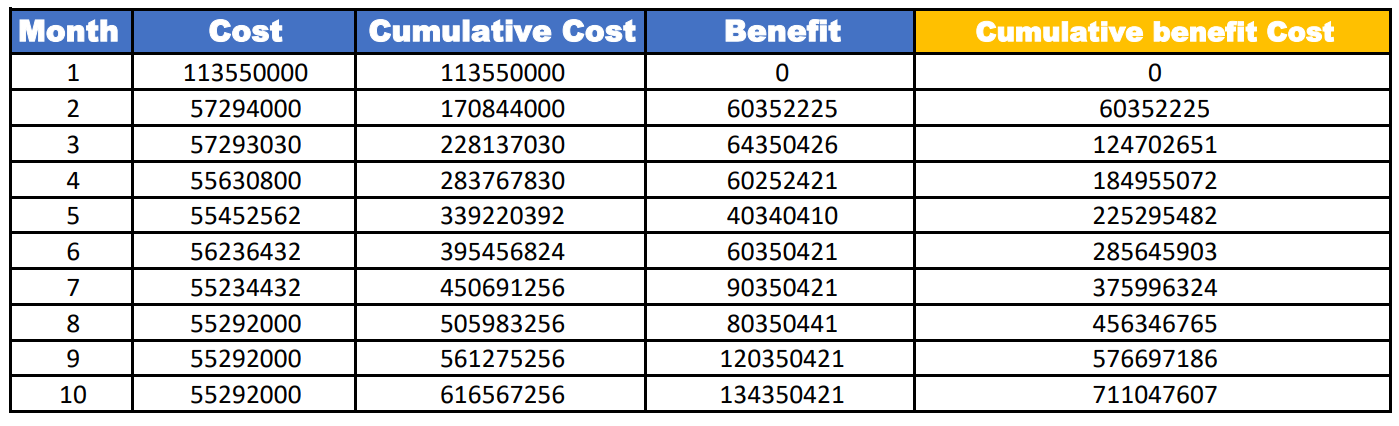
\includegraphics[width=15cm]{img/paybackexel.png}\\
    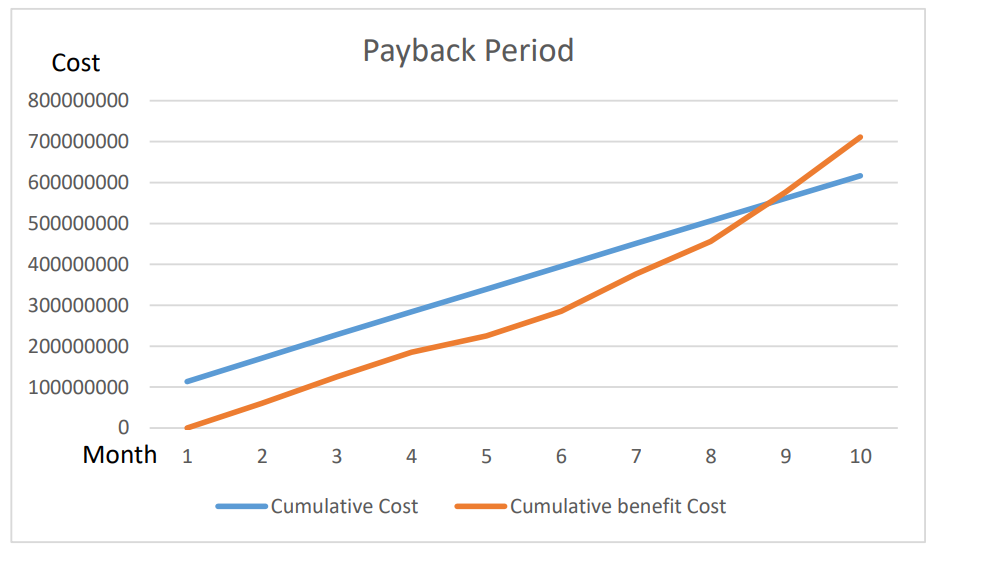
\includegraphics[width=16cm]{img/paybackgraph.png}
    \caption{Payback Period}
    \label{fig:my_label}
\end{figure}

\newpage
\section{UI Design}
\textbf{\Large User Interface of Magpie Composite Textile Ltd Management Software}
\subsection{ Login Page}
\begin{figure}[h]
    \centering
    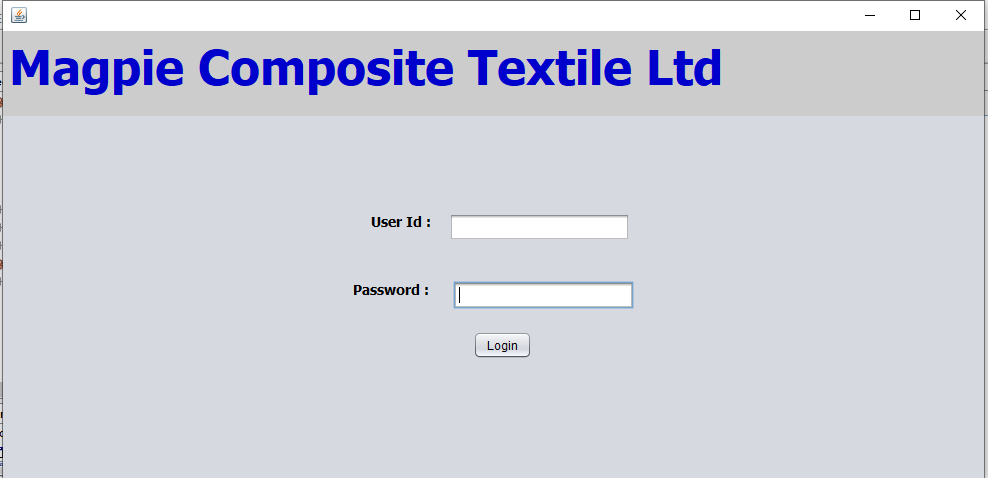
\includegraphics[width=15 cm]{ui/loginpage.png}
    \caption{Login Page}
\end{figure}
\newpage
\subsection{Home Page}
\begin{figure}[h]
    \centering
    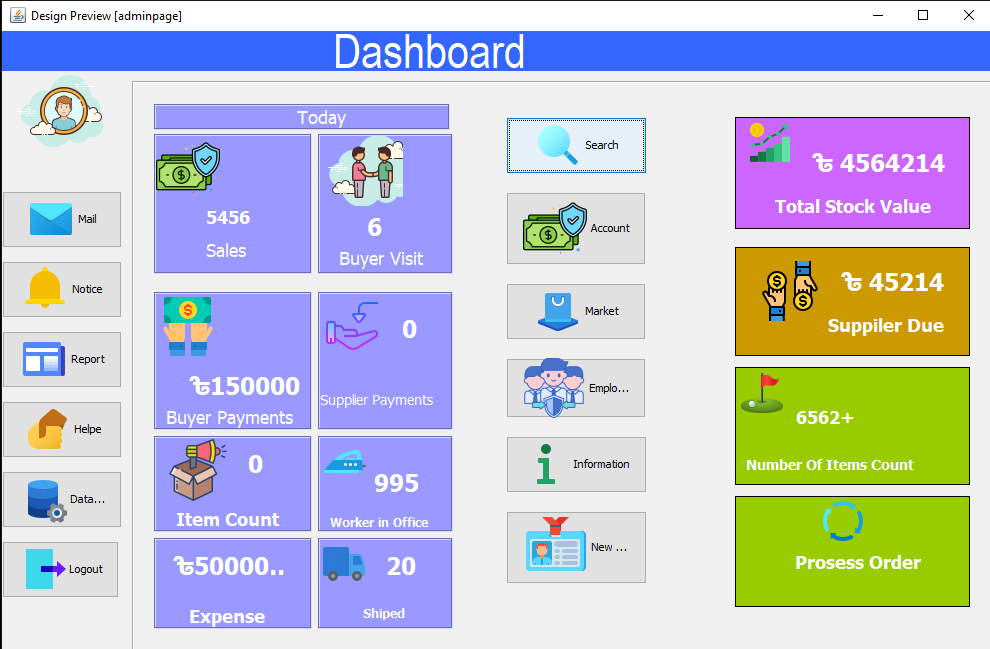
\includegraphics[width=15 cm]{ui/dashboard.png}
    \caption{Dashboard}
    \label{fig:my_label}
\end{figure}
\newpage
\subsection{Employee Information Page}
\begin{figure}[h]
    \centering
    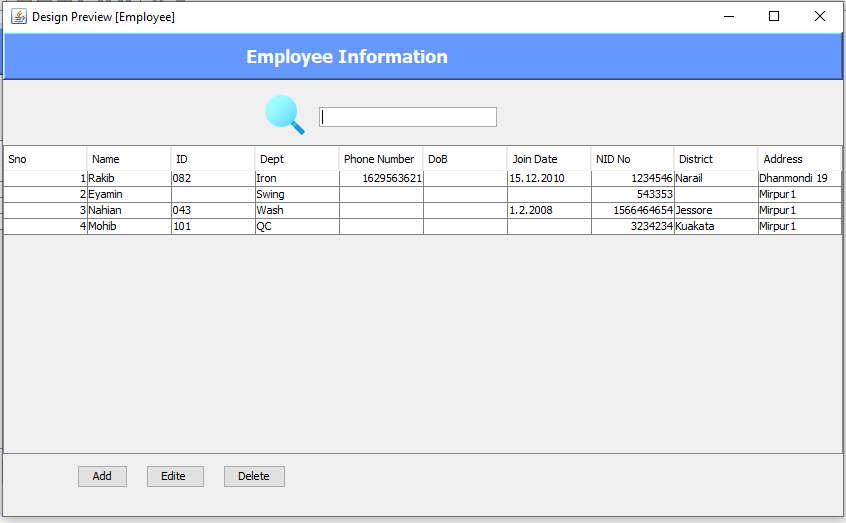
\includegraphics[width= 13 cm]{ui/employeerInfor.png}
    \caption{Employee list}
    \label{fig:my_label}
\end{figure}
\newpage
\subsection{Add Product Page}
\begin{figure}[h]
    \centering
    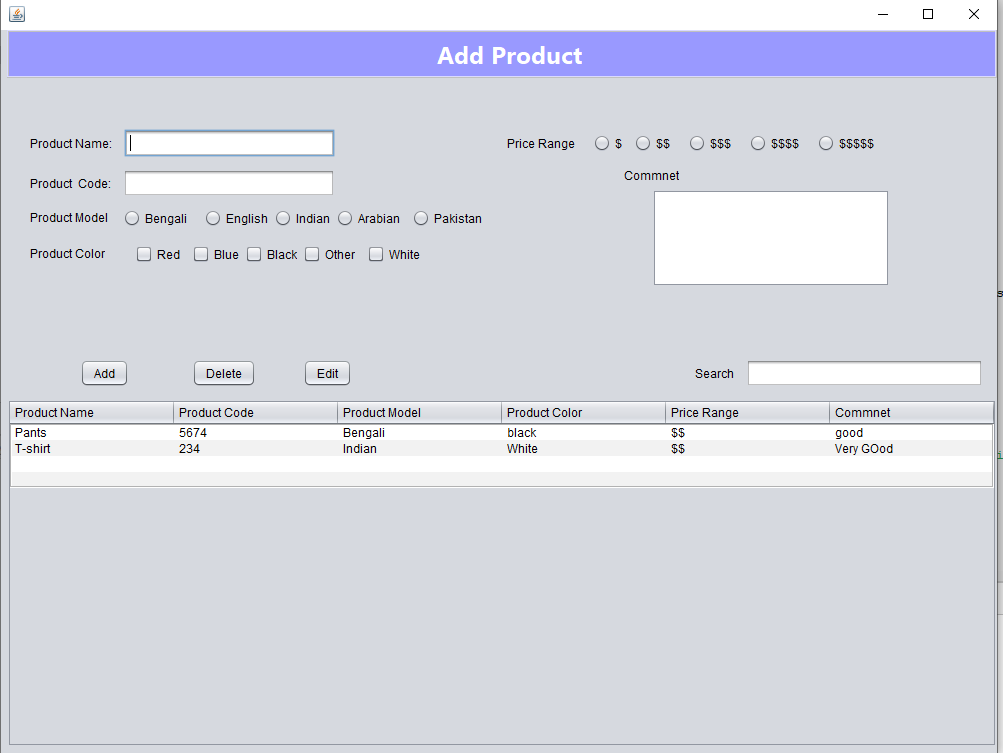
\includegraphics[width=13 cm]{ui/addproduct.png}
    \caption{Add Product}
    \label{fig:my_label}
\end{figure}
\newpage
\subsection{Stock List}
\begin{figure}[h]
    \centering
    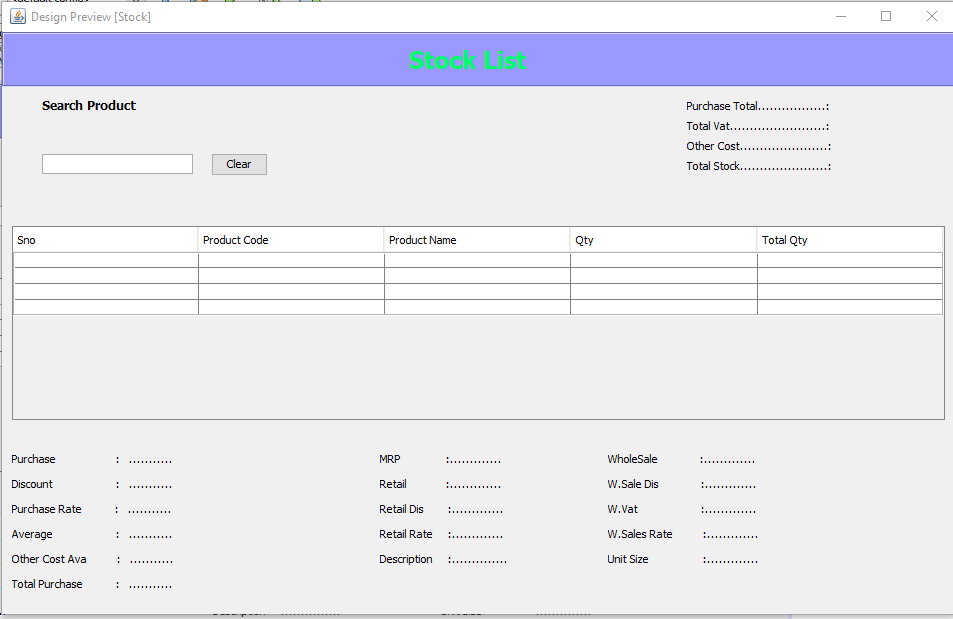
\includegraphics[width=15 cm]{ui/stocklist.png}
    \caption{Stock List}
    \label{fig:my_label}
\end{figure}
\newpage
\subsection{Employee Salary}
\begin{figure}[h]
    \centering
    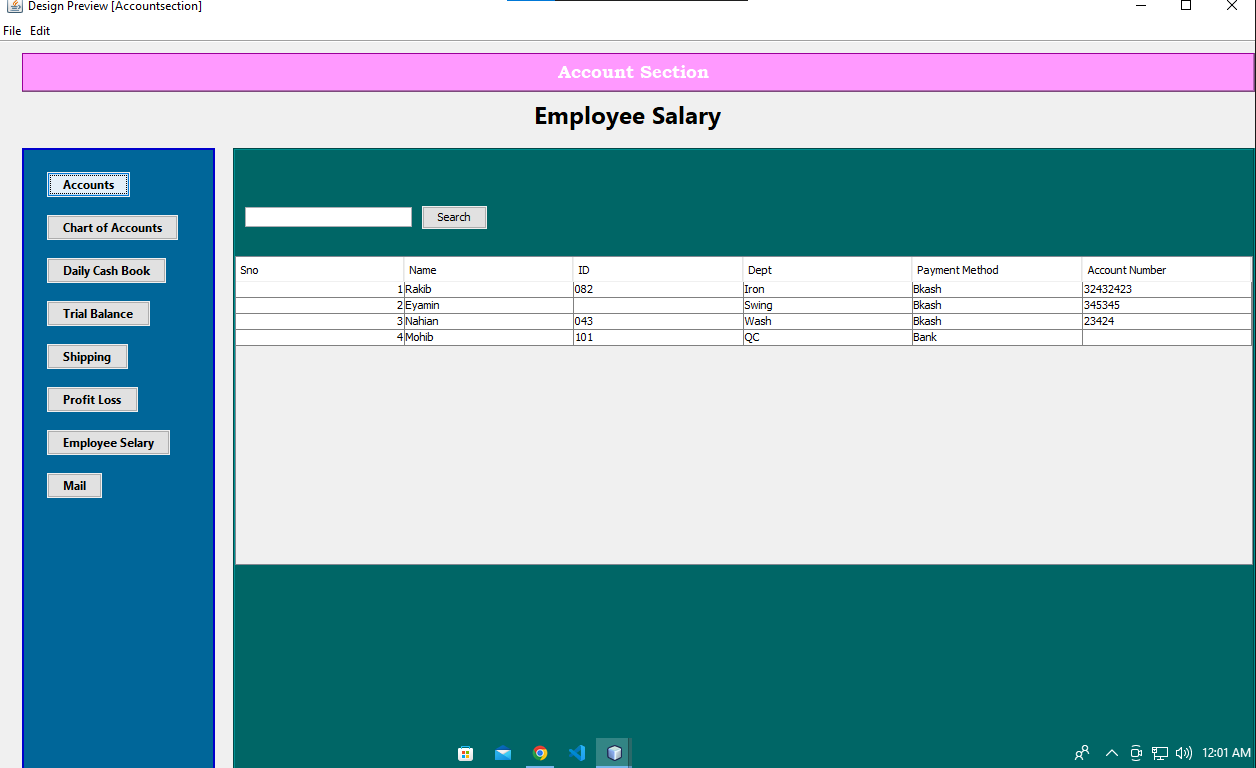
\includegraphics[width=13cm]{ui/selary.png}
    \caption{Salary Page}
    \label{fig:my_label}
\end{figure}

\newpage
\section{Conclusion}
\begin{itemize}
    \item MAGPIE COMPOSITE TEXTILE LTD  is a well-planned versatile project. The administration, management, and chain of command – all are well organized. They are devoted to satisfying the customer through their activities.  
\item The RMG sector plays a key role in the progress of industrial development in Bangladesh.
\item The future growth of  garment factories is mainly  dependent on a collective effort of producers, buyers, policymakers, and a strong  supportive role of the government.
\item, However, some of the points we want to mention for the good of MAGPIE COMPOSITE TEXTILE LTD
\end{itemize}
.






\end{document}
